Intrusive magmatism  is a major  process at  the scale of  a planetary
body and play a fundamental role  in the accretionary processes of the
terrestrial crust. However,  it takes  place deep beneath  the surface  and remain
difficult  to study  without  a proper  model  for magmatic  intrusion
emplacement.  The objective of this thesis was two-fold: to characterize the
dynamics of  a cooling  magmatic intrusion  and to  shed light  on the
origin of floor-fractured craters. 

\section*{Dynamics of shallow magmatic intrusions}

\subsection*{Summary}
\label{sec:summary}

Intermediate-scaled  shallow  magmatic  intrusions  are  the  building
blocks    of    larger    plutons     intruded    into    the    crust
\citep{Petford:2000cc,Glazner:2004gv}.  We show in Chapter \ref{chap1}
that  the topographic  deformation  that could  be  caused by  shallow
intrusions can  be constrained by observations  of planetary surfaces;
that  is, volume,  shape and  other  dimensions of  intrusions can  be
quantified. These  observations have  been previously  used to  draw a
first view of their formation.  However, they must be linked to models
of magma  intrusion dynamics in  order to provide insights  into magma
physical properties and injection rate.

\citet{Michaut:2011kg}  provides  a  consistent $2D$  model  for  such
elastic-plated  gravity current  intrusions  which  directly link  the
observed  deformations  to  physical  parameters of  the  magmas.   In
particular, depending mainly  on the injection rate  and the intrusion
depth, two regimes of propagation  are identified and characterized by
specific morphologies and scaling  laws for intrusion thickness versus
length and time.   In Chapter \ref{chap2}, we develop the  model in an
axisymmetric  geometry  and  compare  the  model  predictions  to  the
morphology  of several  terrestrial shallow  magmatic intrusions.   We
show that  laccoliths and  low-slope lunar  domes are  consistent with
their arrest in the early times bending regime. In addition, the model
predictions    are     consistent    across     different    planetary
settings. However, the absolute dimension of these magmatic intrusions
is  underestimated  by  the  model;  in  particular,  abnormally  high
viscosity are required to reconcile both observations and predictions.

To get  some insight in  the effective  flow viscosity, we  provide in
chapter \ref{C3-JFM}  and \ref{Heating} an  extension of the  model of
\citet{Michaut:2011kg}   that  accounts   for  the   cooling  of   the
elastic-plated gravity current.  We show that the coupling between the
temperature field and  the flow itself results  in important deviation
from the  isoviscous case. In  particular, in the bending  regime, the
effective flow viscosity is governed by the local thermal condition at
the tip of  the current; as the fluid is  cooling, the thermal anomaly
detaches  from  the  tip  and the  flow  effective  viscosity  rapidly
increases   to  stabilize   when   it  reaches   its  maximum   value.
Applications  to   terrestrial  laccoliths  indeed  show   that  their
dimensions are  in agreement  with their arrest  in the  third bending
phase.  A  phase diagram as a  function of the Peclet  number $Pe$ and
the viscosity  contrast $\nu$ is  provided which allows  to constrains
the parameters of the intrusions  given its composition.  We then show
that lunar intrusive domes have  probably been characterized by larger
injection rate  than on Earth,  though much smaller than  the effusion
rates estimated from the runnout distance of some lunar lava flows.

In chapter \ref{Heating},  we proposed that the entrance  in the third
phase  of both  regimes might  have  triggered the  arrest of  shallow
magmatic intrusions.  However, even for laccoliths, we have shown that
conduction cooling  alone is probably  not a sufficient  mechanism for
their arrest,  neither on Earth, nor  on the Moon. Available  data for
large mafic  sills on Earth  also show  less agreement with  the model
prediction.   Indeed, in  chapter \ref{C3-JFM}  and \ref{Heating},  we
show that sills  should behave as isoviscous gravity  current when the
thermal anomaly is small compared to the flow itself, i.e.  in similar
settings, their thickness should tend  to a constant.  The increase in
thickness with diameter preserved in  the data might thus suggest that
they  instead stop  in the  second gravity  phase. However,  the model
lacking of a  stopping criteria for the flow, this  hypothesis can not
be tested properly. In the end, while the cooling of the intrusion has
allowed us to predict the mean in the observations, a complete picture
of the  solution, in regard to  the final radius and  thickness of the
intrusion as a  function of the parameters of  the problem (elasticity
and toughness of the host rock, viscosity of the magma, injection rate
of  the feeder  dyke,  and depth  of emplacement),  has  yet not  been
obtained.

\subsection*{Perspectives}
\label{sec:perspectives}

In Chapter  \ref{chap2}, \ref{C3-JFM} and \ref{Heating},  we show that
the  dynamics  in  the  bending  regime is  controlled  by  the  local
condition at  the tip of  the current.  For  a sake of  simplicity, we
used a thin prewetting film at the tip to avoid the requirement of any
boundary condition at a genuine front.  While this approach allowed us
to get  insights into the  coupling between the thermal  structure and
the flow  itself, a more  precise characterization of the  front might
help predict the final morphology of laccoliths.

\subsubsection*{Detail description of the tip}
\label{sec:caref-descr-tip}

A first step  could be to describe  the tip in term of  a fluid driven
fracture  instead of  the thin  prewetting  film. As  seen in  Section
\ref{C2-Toughness},  linear elastic  fracture mechanics  requires that
the  mode $I$  intensity  factor  $K_I$ equal  a  critical value,  the
fracture toughness  $K_{Ic}$ for  the propagation to  occur, condition
that is  usually expressed in term  of an asymptotic condition  on the
crack                 opening                 at                 $r=R$
\citep{Savitski:2002gy,Bunger:2005em,Bunger:2007vs,Detournay:2014fk}.
In  such  problem, the  lubrication  equation  is  thus coupled  to  a
description  of  the fracture  opening  based  on the  linear  elastic
fracture mechanics.  \citet{Bunger:2011cb} use  this approach to solve
the problem  of shallow magmatic  intrusion and found  similar results
than  \citet{Michaut:2011kg}.  Interestingly,  they needed  values for
the fracture toughness $K_c$ two  or three orders of magnitudes larger
than laboratory measurements in order  to agree with the observations,
which they  attribute to potentially  crack blunting mechanism  at the
tip  of laccoliths.   This observation  is consistent  with the  rapid
cooling  of  the current  tip  describe  in Chapter  \ref{C3-JFM}  and
\ref{Heating}. However, this  model also falls short  to reproduce the
geometry  of large  mafic  sills. In  addition,  more realistic  model
should  also  address  the  question of  plastic  deformation  in  the
fracture       potentially      caused       by      the       heating
\citep{Bunger:2008cl}. Furthermore,  the large negative  pressure that
developed at the front might cause desolved gasses to exsolve from the
magma.  With the formation and the  evolution of a gap filled with gas
at the  tip of the  current, the fluid and  the fracture front  do not
coincide with one  another, thus requiring the tracking  of two moving
boundaries.

Along      with      the     prewetting      film      regularization,
\citet{Anonymous:QWXp_4JV} propose  a second  regularization condition
where the tip of the elastic-gravity  current consists of a lag region
filled   with    gas   at    constant   negative    pressure   (Figure
\ref{C7-Sketch}).   They show  that the  solution depends  on the  gas
pressure  in the  tip  region  in similar  fashion  that the  solution
depends  on  the prewetting  film  thickness  in Chapter  \ref{chap2},
\ref{C3-JFM} and \ref{Heating}.
\begin{figure}[htpb]
  \begin{center}
    \graphicspath{ {/Users/thorey/Documents/These/Manuscript/Figure/Chapter7/} }
    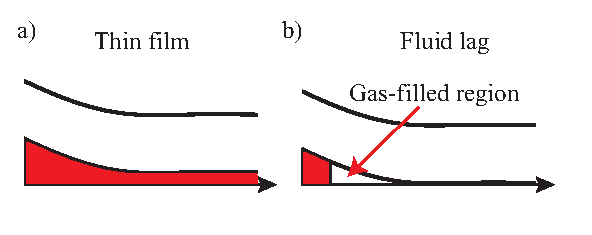
\includegraphics[scale=1.3]{Sketch.eps}
    \caption{Two different  regularization condition  at the  front of
      the current: a) thin prewetting film with thickness $h_f$ b) gas
      -filled region.}
    \label{C7-Sketch}
  \end{center}
\end{figure}
In particular, they show that
\begin{eqnarray}
  h_0&\propto& h_f^{-1/7}\nu^{-2/7}L^{10/7}~(\text{Thin film})\\
  h_0&\propto& \sigma^{1/9}\nu^{-2/9}L^{14/9}~(\text{Fluid lag})
\end{eqnarray}
where $L$  is the half  length of the  flow, $-\sigma$ is  the contant
negative  pressure  in  the  fluid   lag  and  we  have  rescaled  the
characteristic    thickness    and     time    by    $\nu^{1/4}$    in
\citet{Anonymous:QWXp_4JV}.    As   expected,    the   two   different
regularization condition leads  to only minor change  in the thickness
to   length   relationship   ($10/7\sim  1.4$,   $14/9\sim   1.5   $).
Nevertheless, a  complete description of  the dynamics of  the cooling
gas-filled region, whose property are expected  to vary a lot with the
temperature, might also be required.

In the end, further works should  coupled the model derived in Chapter
\ref{C3-JFM} and  \ref{Heating} to a  more careful description  of the
different processes  involves at  the scale of  the current  tip. Such
approach should surely  give interesting insights and  a more complete
view of the dynamics of shallow magmatic intrusion.

\subsubsection*{Contact zone}
\label{sec:caref-descr-tip}

In chapter \ref{Heating},  we show that a  significant thermal aureole
should develop in the wall rocks above the central flow region.  Apart
from  plastic rock  deformation  that might  develop  in the  encasing
rocks,  studying  the  possible  thermal  erosion  could  also  be  an
interesting thing to look at. For instance, above the feeder dyke, the
temperature are  expected to be  maximum on  the roof and  might favor
subsequent dyke propagation. This could potentially explain the nested
structure of  several laccolith  complexes reported in  the literature
\citep{E:2015tl,Rocchi:2010dn}.

\subsubsection*{Multiple magma pulses}
\label{sec:caref-descr-tip}

The  results develop  in this  thesis  mostly account  for a  constant
injection rate $Q_0$. \citet{Michaut:2011kg}  suggests that the weight
of the magma  at the center might compensate  the initial overpressure
$\Delta P$; when $\Delta P/(\rho_m g  H)=h_0$ the flow is thick enough
to accommodate the  overpressure below and enters a  regime of lateral
propagation  \citep{Michaut:2011kg}.   For   the  larger  overpressure
$\Delta P$  and the typical  parameters listed in  Table \ref{C4-tab},
this  would  happen when  $h_0\sim  200$,  which  can be  reached  for
$\nu<10^{-6}$ in the third bending  regime. It would be interesting to
see how  the regime of  lateral propagation  is affected by  the rapid
cooling of the tip.

In  addition, this  model  assumes that  the  overpressure $\Delta  P$
driving magma  ascent remains  constant. For  instance, on  Earth, gas
pressure build up  within the magma chamber is the  most likely source
of overpressure and should decrease  as the magma is evacuated through
the dyke \citep{Rivalta:2010em}.   It would be interesting  to see how
the model developed in Chapter  \ref{C3-JFM} react to a multiple pulse
injection    separated     by    rest    period.      For    instance,
\citet{Macedonio:2014et}   have   used   the   isoviscous   model   of
\citet{Michaut:2011kg}  and show  that the  dynamics of  such multiple
pulse injection fed magmatic intrusion  share similar pattern with the
unrest of volcanic  caldera observed in different  location across the
world.

\subsubsection*{Influence of the topography}
\label{sec:topo}

In Chapter \ref{C5-chap6},  we study the influence of  a depression on
top of the  emplacement zone on the intrusion  dynamics.  Instead, the
model  can be  easily  adapted to  study the  presence  of a  volcanic
edifice.   It  could  then  be   used  to  study  ground  deformations
experienced  by  active volcano  as  a  response  to the  dynamics  of
underground                      magmatic                      systems
\citep{Cayol:2014vo,Pedersen:2004kp,Patane:2006hn,Bonaccorso:2001iw,ChadwickJr:1995cz,Cannavo:2015fk}.

\section*{Lunar intrusive magmatism}

\subsection*{Summary}
\label{sec:summary-1}

While it provides for important  constraints on the Moon's thermal and
petrogenetic evolution,  the total  volume of  melt produced  into the
Moon interior is  poorly known.  Indeed, although  the total extrusive
volume is quantified  through analyses of the lunar  maria, the volume
of intrusive  magma, which should be  large due to the  low density of
the lunar crust,  remains unknown. A first step  in the quantification
of the  intrusive activity  on the  Moon is  the detection  of shallow
magmatic systems.

Low-slope  lunar domes  and floor-fractured  craters are  two proposed
evidences for shallow  magmatic intrusion activity in  the upper lunar
crust. However, these observations must  be linked to shallow magmatic
intrusion models to asses their  intrusive origin.  In this thesis, we
first show that lunar-low slope domes morphology are indeed consistent
with a model  of a cooling magmatic intrusion.   In addition, adapting
the model  of elastic-plated  gravity current model  to account  for a
crater-centered intrusion, we show  in Chapter \ref{C5-chap6} that the
deformations observed  at floor-fractured craters are  also consistent
with  the  emplacement  of  magmatic  intrusions  below  their  floor.
Consistently, taking advantage of the  resolution of the lunar gravity
field  obtained   from  the  NASA’s  Gravity   Recovery  and  Interior
Laboratory  (GRAIL)  mission,  in combination  with  topographic  data
obtained from the Lunar Orbiter  Laser Altimeter (LOLA) instrument, we
show  in Chapter  \ref{chap7} that  their gravitational  signatures is
significantly larger that the one of normal impact craters.

\subsection*{Perspectives}
\label{sec:perspectives-2}


Around  $10$ low-slope  lunar  domes and  about $200$  floor-fractured
craters have been detected at the  lunar surface, most of them located
close  or within  the lunar  maria. While  the total  volume of  these
magmatic intrusion should  not exceed $1\%$ of lunar  maria volume, it
advocates the presence of numerous  shallow magmatic intrusions in the
lunar crust. This  suggests that deeper and  probably larger intrusion
might stands at the base of the lunar crust.

\subsubsection*{Local stress field}
\label{sec:crust-magm-intr}

In Chapter  \ref{C5-chap6}, we argue  that the absence  of deformation
surrounding floor-fractured craters suggests  that the unload pressure
associated with the  crater might have drive magma  ascent below these
craters. However, the unload pressure, associated with the depression,
should  decrease with  depth on  a length  scale equal  to the  crater
diameter, some  tens of  kilometers.  Therefore,  for the  average FFC
diameter, $\sim 30$ km, the depression  caused by the crater can drive
magma flow only if the magma  is already present at depth smaller than
$30$ km, i.e.  within the crust. It thus raises the question of deeper
and larger  magmatic reservoir within  the lunar crust which  might be
observable  in the  the lunar  gravity field  obtained from  the GRAIL
mission.

This idea is also supported by recent works on rift volcanism on Earth
that show that depression can play a crucial role in the trajectory of
magma on the local scale \citep{Maccaferri:2014ft}.  In particular, in
the extensive tectonic setting of rift, \citet{Maccaferri:2014ft} show
the  presence  of   a  stress  barrier,  consequence   of  the  graben
depression, where  $\sigma_3$ turns  to be vertical,  i.e.  preventing
vertical dyke  propagation.  Interestingly,  dyke nucleated  below the
stress  barrier  are  deviated  from  their  vertical  trajectory  and
off-rift  volcanism occur.   While  important  extensive stress  field
should not exist  at floor-fractured crater sites, this  work thus not
favor dykes  initiated deep in  the lunar interior, which  should have
been  deviated  from   the  crater  center,  to   feed  these  shallow
intrusions.

Meanwhile, a  details analysis  of the stress  field below  the crater
depression  could  thus explain  why  these  craters, apart  from  the
underlying low  density breccia,  provide a favorable  environment for
magmatic  intrusions.   At  a  regional scale,  it  could  also  prove
fruitful to investigate  the link between the load of  the lunar maria
and the  distribution of floor-fractured  craters, which is  mainly at
the edge of the maria itself.

\subsubsection*{Thickness of the lunar maria}
\label{sec:crust-magm-intr}

Approximately $16\%$ of the Moon's surface is covered by basaltic lava
flows  that comprise  the lunar  maria. Although  the total  extent of
these lava  flows is  known, their thicknesses  are more  difficult to
constrain \citep{Thomson:2009eo}. Many different approaches, including
indirect  techniques as  gravity,  seismic or  radar  data, or  direct
measurements,  through   analyses  of  impact  that   have  completely
penetrated   the  maria,   have  been   proposed  to   estimate  their
thicknesses.  The  elastic-plated gravity  current models  provided in
this thesis can  also be used to provide estimate  useful to constrain
thickness model of the lunar maria.  Indeed, if the intrusion has stop
in the  bending regime, the  inequality $R<  4\Lambda$ in the  case of
lunar domes or $R<4\Lambda/C$ in  the case of floor-fractured craters,
provide for  an estimate for the  elastic thickness and thus,  a lower
bound for the maria thickness.

\subsubsection*{Floor-fractured craters on other terrestrial planets}

As proven of  the Moon, floor-fractured crater are a  good first basis
to probe the importance of intrusive magmatism on terrestrial planets.
While they  have first been observed  and described on the  Moon, many
evidences  show now  that  floor-fractured crater  might  be a  common
landscape on terrestrial planets.

\begin{figure}[htpb]
  \begin{center}
    \graphicspath{ {/Users/thorey/Documents/These/Manuscript/Figure/Chapter7/} }
    \includegraphics[scale=0.9]{FFCOther.eps}
    \caption{a),  b) and  c) Sample  from the  Marsian FFC  population
      located  respectively  at ($0.0^{\circ}$N,$337.3  ^{\circ}  $E),
      ($5.5^{\circ}$S,$322.6         ^{\circ}          $E)         and
      ($6.7^{\circ}$S,$333.4^{\circ}$E).   All are  TEHMIS daytime  IR
      image taken modified from \citet{Sato:2010ex}.  d) Potential FFC
      on Mercury reproduced from \citet{Schultz:1977ec}.  e) Barrymore
      crater, $50$ km diameter, located near Imdr Regio.  f) Mona lisa
      Crater,  $85$ km  in diameter,  located  on the  edge of  Eistla
      Regio.   Both  are potential  FFCs  on  Venus.  Reproduced  from
      \citet{Wichman:1995ju}.}
    \label{C7-FFCOther}
  \end{center}
\end{figure}

\begin{itemize}
\item  \textbf{Mars}: On  mars, almost  $200$ floor-fractured  craters
  have also been reported located mostly  along a narrow band south of
  the dichotomy boundary in  Arabia Terra \citep{Bamberg:2014hb}.  The
  observed deformations  within these craters  is very similar  to the
  one observed on the Moon, though Marsian floor-fracture craters tend
  to  exhibit a  more  extensive and  wider  fracture network  (Figure
  \ref{C7-FFCOther}  a,  b and  c).   This  is attributed  to  complex
  interaction of  the magmatic  intrusion with potential  ice/water in
  the  subsurface  \citep{Sato:2010ex,Bamberg:2014hb}. In  particular,
  the  melting  of the  water  (or  possibly  CO$_2$) trapped  in  the
  subsurface  would enhance  erosion of  the floor-fractured  which is
  consistent  with   some  small  and  medium   size  fluvial  outlets
  \citep{Sato:2010ex}.    Interestingly,   deformations   on   Martian
  floor-fractured craters is not localized  within the crater wall but
  can  also extend  further the  crater rim  (Figure \ref{C7-FFCOther}
  b,c).   In  contrast  to  the Moon,  the  overpressure  driving  the
  intrusion  might  have  been  larger  than  the  unloading  pressure
  associated with the depression.  In  addition, Martian magma, at the
  difference of their lunar counterpart, are most likely to be buoyant
  until the  surface and  the mechanism  favorable to  intrusion below
  Martian crater is still debated.  Again on Mars, studying the stress
  field associated with  the crater depression could  provide a viable
  mechanism to trigger magma spreading at depth below these craters.

\item   \textbf{Mercury}    \citet{Schultz:1977ec}   propose   several
  candidates  searching for  intra-crater dark  haloes or  other color
  variations  indicating post-impact  emplacement  of mafic  materials
  onto  the  floor.    They  did  find  several   crater  floors  with
  contrasting  deposits,  and  additionally  a  few  rimmed  moat-like
  depression (Figure \ref{C7-FFCOther} d).
  
\item \textbf{Venus}: Venus geologic record  have been largely cut off
  by  resurfacing events  constantly reworking  the Venusian  surface.
  Nevertheless, several candidates have also been proposed on Venus by
  \citet{Wichman:1995ju}.
\end{itemize}

Though most of these observations,  except for Marsian FFCs, have been
made in  the late nineties, they  provide an extremely good  basis for
work using new data  and x new methods at hand  today. In addition, it
provides a  good opportunity to  study and constrain the  important of
shallow intrusive magmatism outside of the Moon.





%%% Local Variables:
%%% mode: latex
%%% TeX-master: "../main"
%%% End:

